\documentclass[french,12pt]{report}
\usepackage[utf8]{inputenc}
\usepackage[francais]{babel}
\usepackage[T1]{fontenc}
\usepackage{lmodern}
\usepackage{ifpdf}
\usepackage{graphicx}
\usepackage{geometry}
\usepackage{color}
\usepackage{pdfpages}

\renewcommand{\familydefault}{\sfdefault}

\geometry{hmargin=50pt, vmargin=50pt}

\title{Rapport de projet : ZigFugl-Meyer}
\author{DYCE William \and MÉLIA Geoffrey}
\date{\today}
\ifpdf
	\pdfinfo 
	{
		/Author (wdyce, gmelia)
		/Title (Title (Rapport de projet))
		/Subject (Subject)
		/Keywords ()
		/CreationDate (\today)
	}
\fi

\begin{document}
	% Page de titre
	%\maketitle
	\thispagestyle{empty}
\begin{picture}(40,40)
\put(50,-600){\rule{.2mm}{21cm}}
\put(-50,-70){\rule{20cm}{.2mm}}

\put(70,-50){\textsc{\Huge{TER : ZigFugl-Meyer}}}
\put(360,-100){\textsc{\Large{Rapport de projet}}}

\put(100,-220){\textbf{\textsc{\large{Étudiants :}}}}
\put(100,-240){\textsc{\large{DYCE William, MÉLIA Geoffrey}}}

\put(100,-400){\textbf{\textsc{\large{Encadrant :}}}}
\put(180,-400){\textsc{\large{SEILLES Antoine}}}

\put(230,-530){\textsc{\large{Master informatique}}}
\put(205,-550){\textsc{\large{Année universitaire 2012-2013}}}
\end{picture}
	
	\thispagestyle{empty}
	\newpage
	
	% Sommaire
	\tableofcontents

	%Table des figures
	\listoffigures
	
	\newpage
	%TODO : grossir, centrer sur la page
	\section*{Remerciements}
	\addcontentsline{toc}{section}{Remerciements}
	\paragraph{}
	
\begin{itemize}
\item Antoine Seilles pour...
\item Ines Di Loreto
\item Julien Métrot et Karima Bakhti (et la jeune patiente) pour ...
\item Isabelle Laffont
\item Benoît Langes
\end{itemize}

\part{Rapport de projet}
\newpage
	\chapter{Introduction}
Les accidents vasculaires cérébraux (AVC) peuvent être la cause d'hémiplégie chez les personnes qui en sont victimes. La paralysie peut affecter une ou plusieurs parties du corps, jusqu'à être totale si la face, le tronc et les membres supérieurs et inférieurs sont paralysés. \\
La récupération des fonctions motrices, de la parole ou de la compréhension dépendent pour beaucoup de l'âge du patient et de son atteinte au niveau du cerveau.
		\section{Problématique}
Il existe de nombreux tests et échelles pour évaluer les capacités sensorimotrices de patients hémiplégiques [\ref {ref_analyse_litterature}]. Cependant, les médecins se retrouvent souvent confrontés au problème de la précision des mesures lors des test. Si la question ne se pose pas pour les tests dits "fonctionnels" (ex : le patient arrive t-il à se servir un verre d'eau?), des mesures d'angles et de positions se révèlent souvent nécessaires pour valider ou non la réussite d'un test par le patient.
\\Or, il existe peu d'outils pour réaliser ces mesures, et ceux-ci ne font pas l'unanimité. Pour la mesure d'angle entre les membres du patient (pli de l'épaule, du coude, etc.), le goniomètre se révèle être l'outil le plus utilisé, mais probablement par défaut (cf \ref{lapeyronie}). On lui reprochera en effet d'être: 
\begin{itemize}
	\item {intrusif :} Il doit être en contact direct avec le patient, pouvant fausser la mesure ou aider/gêner le patient.
	\item {imprécis :} L'épaisseur de peau et de graisse ne permet pas d'évaluer correctement l'angle formé par les os.
	\item {inutilisé :} Des médecins pourtant équipés vont préférer juger à l'œil, pour un meilleur ratio temps/précision.
\end{itemize}
		'une
		\subsubsection{Le test de Fugl-Meyer}
Cette imprécision des mesures devient dès lors gênante lorsque c'est un test non pas fonctionnel, mais de déficience qui est considéré comme le "Gold Standard" dans le domaine : le score de Fugl Meyer [\ref{fugl_meyer}]. En effet, celui-ci consiste à évaluer les mouvements du patient lors de la réalisation de gestes très précis, incluant des mouvements "éliminatoires", qu'il faut donc être capable de mesurer.	
	
	L'idée s'est alors posée d'utiliser un autre moyen de mesure, moins intrusif, pour la réalisation de tests de Fugl Meyer, largement utilisé dans le milieu de la réhabilitation, et de réfléchir aux possibilités d'enrichissement de celui-ci.
\newpage
		\section{Présentation du projet}
		
			\subsection{Étude de terrain} \label{etude_terrain}
		Le projet est avant tout une étude de faisabilité. Nous essayerons de voir
		à quel point nous pouvions procéder, avec un capteur de profondeur (en
		l'occurrence la Microsoft Kinect) et des bibliothèques et outils couramment 
		disponibles, à un test complet ou partiel de Fugl-Meyer.
		
		Nous étudierons donc d'une part les technologies disponibles pour la Kinect,
		et d'autre ce qu'est le test de Fugl-Meyer et quelles sont les 
		problématiques associées.
		
		\subsection{Prototype}
		Nous élaborerons ensuite une preuve de concept,données de tout c'est à dire un 
		prototype proposant au patient en cours de réhabilitation un test partiel 
		de Fugl-Meyer. Les points importants à considérer pour un tel prototype 
		sont~:
		\subsubsection{Automatisation et objectivité}
		Le système doit pouvoir procéder à une évaluation, de manière non-intrusive 
		et sans intervention externe, de ce qui se trouve devant lui. Il doit donc 
		proposer une série de notes objectives qui correspondent aux performances du 
		patient.
		\subsubsection{Aspect ludique~: "gamification"}
		La "gamification" est le processus qui consiste à ajouter des éléments 
		souvent associés au domaine du jeu (d'où le nom), comme des barres de
		progression ou des défis à relever, à une activité non-ludique. L'idée est 
		de favoriser l'implication et la motivation des participants. 
		Notons qu'il ne s'agit pas nécessairement de faire de l'activité en soi un 
		jeu.
    \subsubsection{Retour d'information continue et granulaire}
    La "granularité" d'un retour est le nombre d'options possibles. 
    Chaque exercice du Fugl-Meyer, par exemple, est noté sur trois points. Nous 
    aimerions proposer une alternative plus nuancée.
    L'argument pour le retour d'information rejoint celui de la "gamification"~:
    la notion de "sens" dans un jeu, au moins d'après Salen et Zimmerman, est 
    directement lié à la richesse de ce retour.
    
    % "Rules of Play" on "meaningful play"

	\chapter{Background}
	
	
		\section{Kinect}

			\subsection{Description}
La Kinect, connue à l'origine sous le nom "Project Natal" est une
périphérique informatique créé par Microsoft, comportant une caméra
couleur, un étalage de 4 microphones, des moteurs pour s'orienter avec 
accéléromètres 
et un système senseur de profondeur composé d'un 
projecteur infra-rouge et d'un capteur. 
  \begin{figure}[h!]
  \centering
  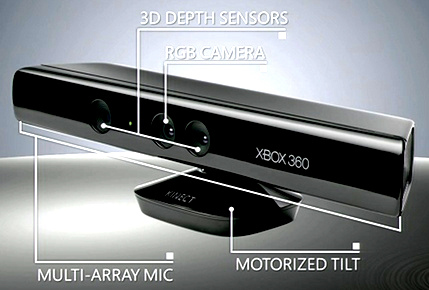
\includegraphics[width=0.8\linewidth]{images/kinect_diagram}
  \caption{Diagramme montrant les sous-systèmes de l'appareil Kinect.}
  \end{figure}
L'appareil n'utilise pas, comme on pourrait croire, le "Temps de Vol" pour
calculer la profondeur d'une scène. C'est en fait la déformation de chaqu'un de 
sa matrice de rayons infra-rouge,
lorsqu'ils frappent une surface, qui est mesuré. Cette technique dite de 
"Lumière Structuré"
lui permet de générer une image 3D d'une scène à une résolution de 640x480 avec 
une profondeur de 11 bits, qui sera mise à jour 30 fois par seconde.

			\subsection{Historique}
Sorti en Novembre 2010, le système était prévu à l'origine pour la console
de jeu de Microsoft, la "Xbox360". Comme la plupart des consoles et
périphériques de jeu elle
est donc vendu à perte, l'idée étant de récupérer l'argent perdu en vendant
des jeux. Ceci en fait l'appareil de son genre le moins cher et le plus couramment
disponible.

Il est donc peu surprenant que, dès sa sortie, des pilotes Libres et gratuits
ont été créés afin de permettre le détournement du périphérique par des
chercheurs et des amateurs. Microsoft a répondu en début de 2011 avec un
premier SDK pour Windows initialement peu complet. Des mises à jours et une
deuxième version, sortie en Octobre 2012, comblent ces lacunes.

		
		\section{Aspect médical} \label{lapeyronie}		%---GEOFFREY---
		% je commente, car je ris à chaque fois que je lis cette ligne :
%		PARLER DES DUDES QU'ON A RENCONTRE A PERLARONIE
Ce projet, d'un choix assumé par les étudiants et la société NaturalPad qui en est l'inspiratrice, comporte une composante recherche forte. C'est dans cette optique et comme expliqué en \ref{etude_terrain} que nous avons commencé notre projet par un travail d'investigation et de recherche d'informations. Dans ce but, nous avons rencontré des praticiens de l'hôpital Lapeyronie à Montpellier : Julien Métrot, doctorant du Laboratoire Movement To Health et Karima Bakhti, kinésithérapeute au CHU de Montpellier. Lors de cette entrevue, ils ont partagé avec nous leurs connaissances sur le test de Fugl Meyer et bien plus encore, et nous ont offert la possibilité d'assister à la réalisation d'un tel test sur une patiente atteinte d'hémiplégie.
	\subsection{Fugl Meyer}
Le test de Fugl Meyer constitue un ensemble d'exercices à effectuer par le patient, et dont chaque mouvement est évalué selon un ou plusieurs critères, fournissant un score généralement compris entre 0 [échec], 1 [intermédiaire] et 2 [réussite]. Ces exercices peuvent concerner successivement les membres inférieurs et supérieurs, eux même divisés en sous catégories. Pour les membres supérieurs, on notera la présence d'un score \textit{proximal} et d'un score \textit{distal}. Ce test a pour vocation d'être réalisé régulièrement tout au long de la période de réhabilitation du patient, afin de mesurer ses progrès.
	\subsection{Réalisation du test}
				\subsubsection{Contexte}
Nous avons assisté à la passation d'un test de FM sur une jeune patiente atteinte d'une hémiplégie suite à un AVC ; ses membres supérieurs droits étaient affectés. Comme nous l'ont précisé J. Métrot et K. Bahkti, seules les parties du test concernant les membres supérieurs ont donc bien sur été réalisées. Pour les détails des mesures et exercices effectués lors de ce test, se référer à l'annexe \ref{evaluation_FM}.

				\subsubsection{À noter}
Les patients concernés par la rééducation des membres supérieurs, comme la patiente qui a accepté de passer 
le FM en notre présence, sont globalement plus nombreux. Cela concorde avec les contraintes du capteur Kinect, 
qui possède un petit angle de vue. Il est alors nécessaire d'avoir beaucoup d'espace (de recul) dès lors que 
l'on souhaite capter l'intégralité d'une personne de manière précise. \\
Lors des tests, le médecin ou personnel médical chargé s'occupant du patient, peut être amené à 'aider' celui-ci.
Cela peut se traduire, outre les éventuels encouragements oraux, en maintenant ou en bloquant un membre du patient
non directement concerné par l'exercice du test. Par exemple, lorsque l'on demande au patient de "tourner son avant 
bras" (prono-supination de l'avant bras) avec le bras tendu, le praticien peut aider le patient à maintenant son bras
(partie haute).\\
Notons aussi qu'en l'occurrence, les praticiens n'ont pas eu besoin d'utiliser de goniomètre ou autre instrument de 
mesure pour évaluer la qualité des gestes de la patiente.
		
	\subsection{L'avis des professionnels}
	Le test de Fugl Meyer est le plus répandu et accepté : il constitue le "gold standard" dans le milieu.
	Nos interlocuteurs regretteront toutefois une certaine subjectivité et interprétation des résultats.
	Nous en avons d'ailleurs eu une démonstration lors de ce test : il arrivait que K. Bahkti et J. Métrot 
	évalue différemment les mouvements de la patiente. \\
Une autre critique est "l'effet plateau" qu'induit ce test. En effet, l'échelle de mesure est très petite 
(2, maximum 3 valeurs de notation) et le patient atteindra régulièrement des 'seuils' sur son score global. 
C'est-à-dire que même si il réalise encore des progrès par rapport aux fois précédentes, cela ne se pas forcément 
visible et impactant sur le score global, à cause du manque de granularité de la mesure. Même si cela n'est pas une 
fin en soi, on peut noter l'aspect peu encourageant que cela peut apporter au patient. \\
Pour les mêmes raisons, le patient pourra obtenir un score maximal (dans notre étude de cas, 66/66) sans pour autant
avoir recouvré la totalité de ses capacités, et quand bien même des progrès sont encore possibles. \\
Cela amène au regret que le test standard soit un test jugeant la \textbf{déficience} et non la \textbf{fonctionnalité}. 
Il existe cependant de nombreux autres tests, et une des alternatives intéressante est le test "ARAT : 
Action Research Arm Test". %TODO réf lien
Rapidement, ce test consiste à vérifier si un patient est capable d'effectuer un geste du quotidien (déplacer
un objet, se servir un verre d'eau, etc), et de chronométrer le temps que cela lui a pris. C'est donc un test 
de fonctionnalité.
	
	\subsubsection{Impressions et propositions}
Après notre entretien et cette passation du test de FM, et à partir de nos tests préliminaires, nous en avons 
conclu que l'utilisation du kinect semblerait plus adpatée pour faire une évaluation des performances “proximales”.
En effet, la taille des membres et l'amplitude des gestes requis pour l'évaluation proximale offrent de bien 
meilleures possibilités d'analyse des mouvements. Certains gestes du poignet semblerait aussi bien adaptés.
\paragraph{}En revanche, les autres mouvements distaux semblent trop difficile à percevoir et interpréter par le capteur.
L’idée serait de proposer une évaluation de grain plus fine, allant au délà d’une évaluation trinaire entre 
“a réussi à lever le bras à l’horizontal”, “a levé son bras partiellement” et “n’a pas réussi à lever son bras”. 
Il serait utile de pouvoir donner l’angle exact, par exemple.   

\paragraph{}Les tests sur la main sont évalués de manière “tactile” (tests de résistance, de préhension) pour la plupart, 
avec peu de différence visuelle entre une évaluation 0 et 2. L’utilisation de la Kinect semble alors peu pertinente
pour cette partie de l’évaluation.
		
	\chapter{État de l'art}
	
  \section{Bibliothèques Kinect}
  \section{La Microsoft Kinect}

\subsection{Description}
La Kinect, connue à l'origine sous le nom "Project Natal" est une
périphérique informatique créé par Microsoft, comportant une caméra
couleur, un étalage de 4 microphones, des moteurs pour s'orienter avec 
accéléromètres 
et un système senseur de profondeur composé d'un 
projecteur infra-rouge et d'un capteur. 
  \begin{figure}[h!]
  \centering
  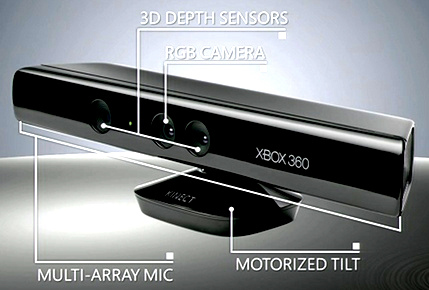
\includegraphics[width=0.8\linewidth]{images/kinect_diagram}
  \caption{Diagramme montrant les sous-systèmes de l'appareil Kinect.}
  \end{figure}
L'appareil n'utilise pas, comme on pourrait croire, le "Temps de Vol" pour
calculer la profondeur d'une scène. C'est en fait la déformation de chaqu'un de 
sa matrice de rayons infra-rouge,
lorsqu'ils frappent une surface, qui est mesuré. Cette technique dite de 
"Lumière Structuré"
lui permet de générer une image 3D d'une scène à une résolution de 640x480 avec 
une profondeur de 11 bits, qui sera mise à jour 30 fois par seconde.

\subsection{Historique}
Sorti en Novembre 2010, le système était prévu à l'origine pour la console
de jeu de Microsoft, la "Xbox360". Comme la plupart des consoles et
périphériques de jeu elle
est donc vendu à perte, l'idée étant de récupérer l'argent perdu en vendant
des jeux. Ceci en fait l'appareil de son genre le moins cher et le plus couramment
disponible.

Il est donc peu surprenant que, dès sa sortie, des pilotes Libres et gratuits
ont été créés afin de permettre le détournement du périphérique par des
chercheurs et des amateurs. Microsoft a répondu en début de 2011 avec un
premier SDK pour Windows initialement peu complet. Des mises à jours et une
deuxième version, sortie en Octobre 2012, comblent ces lacunes\cite{wiki_kinect}.

\subsection{Pilotes et bindings bas-niveau}

Il est important de noter que la reconnaissance vocale et l'extraction de 
squelette ne sont pas faits par l'appareil, ou "serveur", lui-même~: ce sont des
bibliothèques sur la console ou l'ordinateur, le "client", qui s'en chargent. 
Il faut donc bien
différencier les pilotes de bibliothèques de bas niveau, qui permettent 
d'accéder aux données brutes, des
bibliothèques de haut-niveau, qui interprètent ces données.

Le jour de la sortie de la Kinect, le 4 Novembre 2010, Adafruit Industries 
offre une prime de \$2000 (augmentée ensuite jusqu'à \$3000) pour le premier qui
sortira des pilotes permettant l'utilisation de la Kinect sur ordinateur\cite{adafruit_bounty}.

\subsubsection{Libfreenect}
\begin{figure}[h!]
\centering
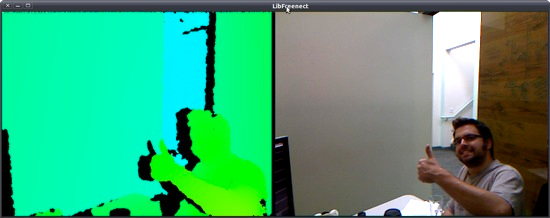
\includegraphics[width=\linewidth]{images/hector}
\caption{Première sortie de la Libfreenect par son créateur, Hector.}
\end{figure}
Le prix est remporté 6 jours plus tard le 10 Novembre par un programmeur Linux
connu sous le nom "Hector"\cite{adafruit_winner}. C'est la première version de Libfreenect autour
duquel le groupe OpenKinect se forme. Libfreenect a pour avantage son
très grand nombre de bindings~: C/C++, Java, Python, Actionscript, Javascript,
LISP, C\#, pour ne nommer qu'un sous-ensemble. 
Il est toujours maintenu (dernier commit Décembre 2012).
\begin{figure}[h!]
\centering

\includegraphics[width=0.5\linewidth]{images/openkinect_logo}
\caption{Logo de la OpenKinect.}
\end{figure}

\subsubsection{CL NUI}
9 jours après la sortie de Libfreenect la compagnie Coding Laboratories 
(CL) et le groupe logiciel-libre
Natural User-Interaction (NUI) sortent CL-NUI\cite{clnui}. Nous sommes alors 2 semaines 
après la sortie de l'appareil. CL-NUI propose des bindings 
WPF\footnote{Windows Presentation Foundation}/C\# C et C++ et permet d'accéder 
à tout sauf le microphone. Le développement continue jusqu'en fin Décembre 2010 
mais,
le défi déjà remporté, s'arrête par la suite. Notons pourtant qu'il faudra 
attendre 2 ans pour avoir accès aux données des accéléromètres à travers la 
SDK officiel\ldots
\subsubsection{Kinect for Windows}  
Les pilotes officiels de Microsoft viennent avec leur SDK, "Kinect for 
Windows". Inutile de dire
qu'ils ne fonctionnent que sous Windows. Ce qui est un peu plus surprenant 
c'est qu'il n'y a de soutient que pour Window 7 et 8, donc pas pour Windows XP 
ou Vista.
\subsubsection{SDK OpenNI}
OpenNI (Open Natural Interaction) est un consortium à but non lucratif composé
des grands acteur économiques du domaine. S'y figure notamment PrimeSense, la 
compagnie qui a développé la Kinect pour Microsoft au premier lieu. Leur SDK
est plus ou moins analogique à celui de Microsoft où il est question de
Kinect, mais fonctionne aussi sur les plus anciennes 
versions de Windows mais
aussi sous Linux (y compris Android) et Mac OSX.
\begin{figure}[h!]
\begin{minipage}{0.49\linewidth}
  \centering
  
\includegraphics[width=0.9\linewidth]{images/openni_logo}
\end{minipage}
\begin{minipage}{0.49\linewidth}
  \centering
  
\includegraphics[width=0.9\linewidth]{images/primesense_logo}
\end{minipage}

\caption{Logos de la OpenNI et de PrimeSense.}
\end{figure}
La OpenNI permet également de s'abstraire du matériel utilisé. Il suffit que
les pilotes utilisés soient conformes à ses standards~: pour passer, par 
exemple, de la Kinect à une caméra PrimeSense nous devons simplement remplacer 
les pilotes "SensorKinect" avec "PrimeSensor".
\begin{figure}[h!]
\centering
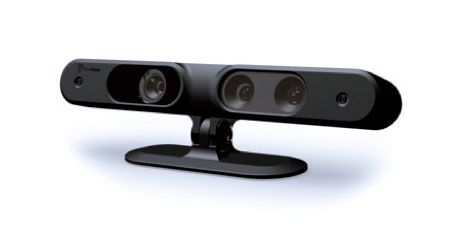
\includegraphics[width=0.6\linewidth]{images/primesense_camera}
\caption{Caméra Carmine 1.09 de PrimeSense.}
\end{figure}

% ------------------------------------------------------------------------------  

\subsection{Middleware}
Les bibliothèques dites "middleware interaction naturelle" servent ici en 
générale à faire une 
extraction de squelette et une reconnaissance de gestes. Elles permettent donc 
au développeur de s'abstraire des données brutes. Le groupe OpenNI définit 
des normes auxquelles doivent obéir cette couche, de 
manière à faciliter la communication à travers la pile de technologie (voir 
figure~\ref{fig:openni_technology_stack}).
\begin{figure}[h!]
\centering
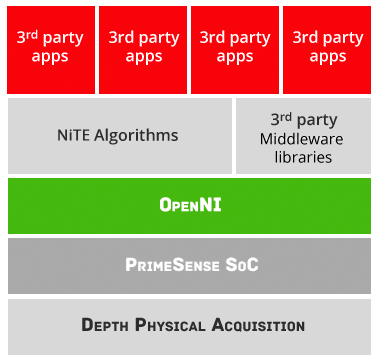
\includegraphics[width=0.7\linewidth]{images/openni_technology_stack}
\caption{Pile de technologie d'après la OpenNI.}
\label{fig:openni_technology_stack}
\end{figure}


\subsubsection{Kinect for Windows}  
Bien que les SDK de Microsoft et de la OpenNI signifient tout deux 
"Simple Development Kit",
celui de Microsoft, "Kinect for Windows", contient à la fois les pilotes, 
l'API de bas niveau et une couche d'analyse des données qu'OpenNI appellerait 
middleware. Il n'est donc pas fait pour interfacer avec les couches de la 
OpenNI et donc ne suit par leur normes.

Kinect for Windows a quelques avantages par rapport à NITE~: il propose un
placement prédictif des articulations et génère deux points en plus :
le poignet et le bout des doigts. Cela étant sa prédiction consomme beaucoup 
plus de ressources et peut amener à de faux positifs\cite{microsoft_vs_openni}.

\subsubsection{NITE de PrimeSense}
NITE (Natural Interface Technology for End-User) est un framework Libre et 
multiplateforme développé par PrimeSense. Vu que c'est PrimeSense qui a 
lancé OpenNI, NITE est devenu la tête d'affiche de ses
middleware standardisés. Elle se repose donc sur la SDK de la OpenNI. 
\begin{figure}[h!]
\centering

\includegraphics[width=0.3\linewidth]{images/nite_logo}
\caption{Logo du framework NITE.}
\end{figure}

\subsubsection{OpenCV}
OpenCV (Open Computer Vision) est une vaste bibliothèque de toutes sortes de 
fonctions aillant un rapport avec la détection de formes à partir d'images
statiques ou dynamiques. Il existe depuis 1999, donc bien avant la Kinect.
\begin{figure}[h!]
\centering

\includegraphics[width=0.4\linewidth]{images/opencv_logo}
\caption{Logo de la OpenCV.}
\end{figure}
Étant donnée qu'il s'agit d'une bibliothèque généraliste il a peu de 
fonctionnalités qui ciblent précisément les données 3D, contrairement aux 
bibliothèques dites "d'interaction naturelle".

% ------------------------------------------------------------------------------  

\subsection{Bibliothèques de haut-niveau}

\subsubsection{Zigfu}
Crée en Mai 2011, Zigfu est une petite entreprise formée de 4 personnes dont 
Amir Hirsch, le fondateur, et 2 ex-employés de PrimeSense. Il fournit, 
par dessus de l'extraction de squelette et de la reconnaissance
de gestes, un API permettant de créer des boutons, listes, curseurs et autres
éléments GUI, tous contrôlés par le mouvement.
\begin{figure}[h!]
\centering

\includegraphics[width=0.3\linewidth]{images/zigfu_logo}
\caption{Logo de Zigfu.}
\end{figure}
Zigfu intègre également la cinématique inverse et un système de 
prédiction et
d'interpolation à fin d'avoir une squelette répondant à des contraintes 
physiques à 60Hz\cite{zigfu_video}. La plupart des jeux moderne tournent à cette 
vitesse, et 
rappelons nous que la caméra ne fournit que des données 30Hz.

Zigfu fonctionne avec Kinect for Windows ou OpenNI avec NITE. Il est 
avant-tout orienté Web, avec des
bindings HTML 5 et Unity, et une version Flash en cours de développement
\cite{zigfu_review}.

\subsubsection{FAAST}
La Flexible~Action~and~Articulated~Skeleton~Toolkit (FAAST) est une 
bibliothèque qui se repose soit sur Kinect for Windows, soit OpenNI et NITE, 
comme Zigfu. Il n'est pour l'instant compatible qu'avec Windows.

Développé par la Interactive~Media~Division (MxR) de 
l'Institute~of~Creative~Technologies (ICT) de 
l'University~of~Southern~California (USC). Il permet de monter à un niveau 
encore plus abstrait~: l'utilisateur travaille avec des événement générés à
partir de postures et des gestes, au lieu d'analyser manuellement la 
squelette.

% ------------------------------------------------------------------------------  

\subsection{Résumé}
Le schéma \ref{fig:technology_overview} résume les interactions entre les divers 
technologies que nous ayons vues.

\begin{figure}[h!]
\centering
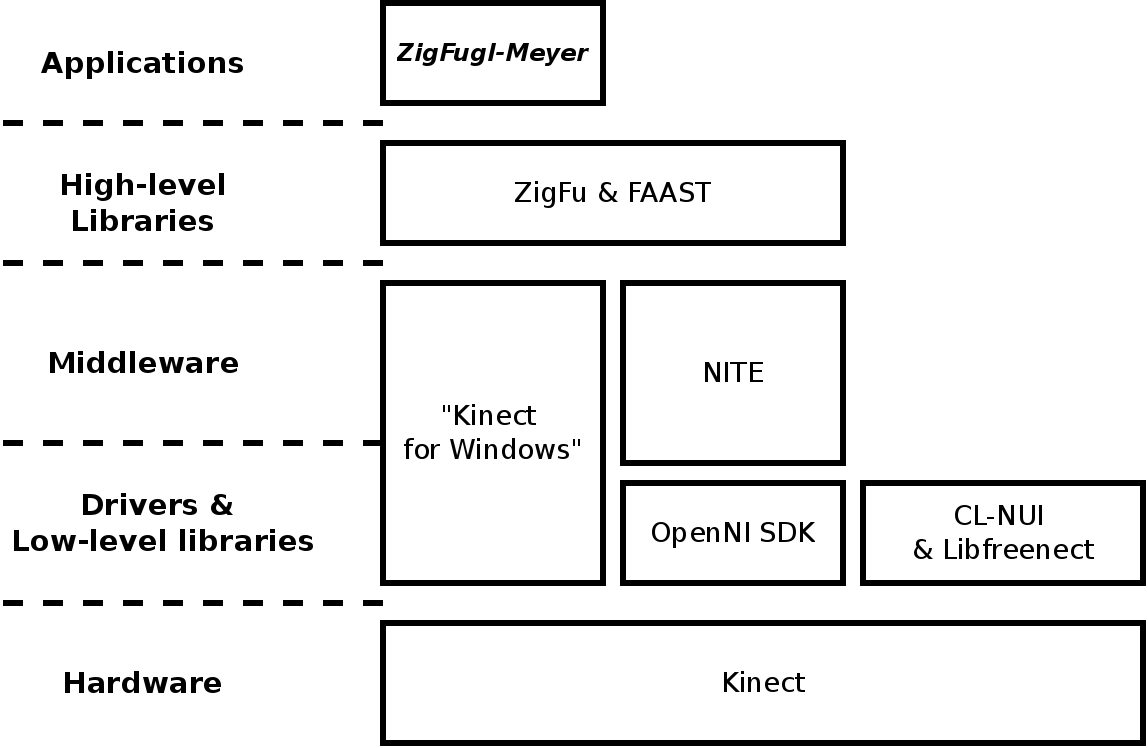
\includegraphics[width=0.9\linewidth]{images/technology_overview}
\caption{Pile de technologie de la Kinect.}
\label{fig:technology_overview}
\end{figure}
  
  \section{"Interaction naturelle" et rehabilitation}
  \section{"Interaction naturelle" et réhabilitation}

\subsection{Applications orientés "fitness"}

\subsubsection{Wii Fit}

Si certains jeu proposaient déjà une interaction naturelle, avec l'EyeToy 
de la Playstation de Sony (2003), la console Wii de Nintendo (2006) est 
l'amorce claire de l'enthousiasme présent vis-à-vis de telles interfaces, et cet enthousiasme va bien
au delà des jeux. 
Si nous avons aujourd'hui la Kinect de Microsoft ou encore la
PS Eye de Sony, c'est grâce au controleur "Wiimote" (voir figure~\ref{fig:wii}), 
capable de reconnaître des mouvements à 
travers l'espace grâce à un système d'accéléromètres. 

\begin{figure}[h!]
\centering
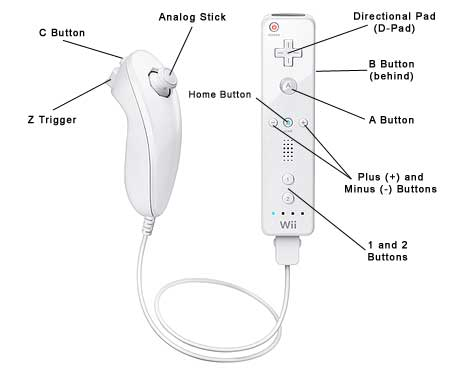
\includegraphics[width=0.7\linewidth]{images/wii_diagram}
\caption{Le controleur de la console Wii de Nintendo.}
\label{fig:wii}
\end{figure}

Avec le jeu Wii Fit, Nintendo ajoute la Wii Balance Board (voir figure 
\ref{fig:balance_board}). C'est un accessoire capable de mesurer le 
poids mis sur chaque pied et donc la position du centre de gravité. Quant au jeu,
il propose un suivi de la remise en forme du joueur à travers des graphiques, 
points et barres de progressions~\ref{fig:wii_fit}~: de la "gamification", 
tout simplement.

\begin{figure}[h!]
\centering
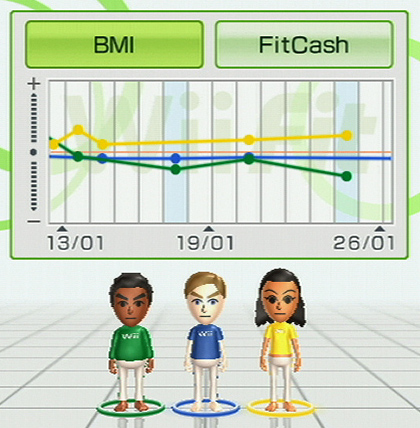
\includegraphics[width=0.5\linewidth]{images/wii_fit}
\caption{Courbes de progression au cours du temps dans le jeu Wii Fit.}
\label{fig:wii_fit}
\end{figure}

\begin{figure}[h!]
\centering
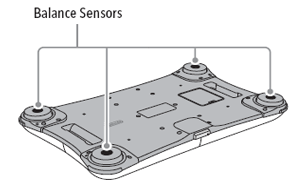
\includegraphics[width=0.5\linewidth]{images/balance_board}
\caption{La Wii Balance Board de Nintendo.}
\label{fig:balance_board}
\end{figure}

\subsubsection{Nike+ Kinect Training}

La Wii est, cela dit, très limitée par son matériel. Un contrôleur peut mesurer
le mouvement d'une main, mais pas sa position absolue. En plus, pour que deux 
mains soient
mesurées il est nécessaire d'avoir un câble de 1 mètre environ entre les deux
contrôleurs~: selon la taille de l'individu cette solution peut ne pas être
idéale. Quant à la Balance Board elle ne perçoit qu'une distribution du poids dans 
le plan, pas la position du corps dans l'espace.

\begin{figure}[h!]
\centering
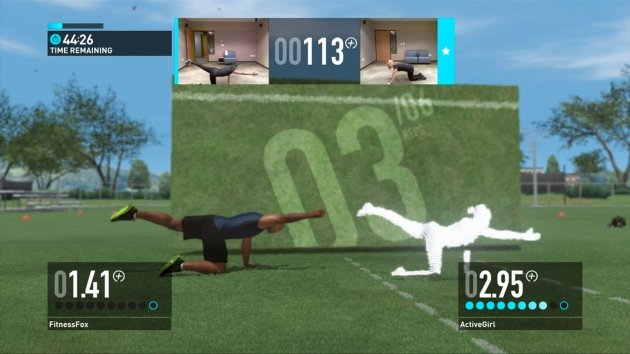
\includegraphics[width=0.8\linewidth]{images/nike_kinect}
\caption{Capture d'écran du "Nike+ Kinect Training".}
\end{figure}

Entre littéralement en jeu la Kinect, périphérique de Microsoft permettant une
extraction non-intrusive du squelette de l'individu. Avec cette technologie
il est possible de mesurer la flexibilité d'un individu et aussi de lui faire répéter
un exercice en vérifiant qu'il a bien été fait. 
Comme pour la Wii Fit, un suivi constant est proposé, avec retour sur
l'amélioration (ou pas) de joueur au cours du temps.


% ------------------------------------------------------------------------------  

\subsection{Quelques applications thérapeutiques}

\subsubsection{"Wiihabilitation"}

Les jeux Wii demandent souvent un mouvement du membre supérieur pour y 
jouer. De ce fait, de nombreuses 
cliniques aux États Unis se sont mis à les détourner à des buts 
thérapeutiques\cite{atwiki_wiihab}. Il s'agit bien ici de "détourner"~: rares sont les cas où des
applications spécifiques sont développées pour ce système par un tiers. Ceci
est probablement du au manque d'outils de développement officiels. Il existe
cependant un très grand nombre d'outils et de bibliothèques non-officiels
\cite{homebrew_wii}, et
c'est d'ailleurs le succès de ces efforts qui a motivé Adafruit à offrir sa prime
pour l'ouverture de la Kinect~\cite{adafruit_bounty}.

\subsubsection{MOJOS}
Lancé en 2010 avec un cycle de développment de 3 ans, 
La Moteur~de~Jeu~Orienté~Santé (MOJOS) est une collaboration entre~:
\begin{itemize}
\item \textbf{professionnels} de DIDACT Systèmes, NetDivision et GENIOUS,
\item \textbf{informaticiens} de l'UM2 et du LIRMM,
\item \textbf{médecins} de l'UM1, du CHU et du centre 
de recherche Efficience et Déficience Motrice (EDM),
\item \textbf{l'IDATE}, \emph{think tank} pour l'innovation numérique.
\end{itemize}

\paragraph{}
Son objectif était de développer un moteur de jeu permettant 
l'élaboration facile d'applications à but thérapeutiques, avec une étude 
expérimentale
par la suite, pour vérifier la pertinence de ces applications~\cite{mojos}. En est sorti 
notamment le jeu Voracy Fish de GENIOUS (voir figure~\ref{fig:voracy_fish})
qui propose un exercice du membre supérieur~: le patient contrôle un poisson 
vorace grâce à une Kinect.

\begin{figure}[h!]
\centering
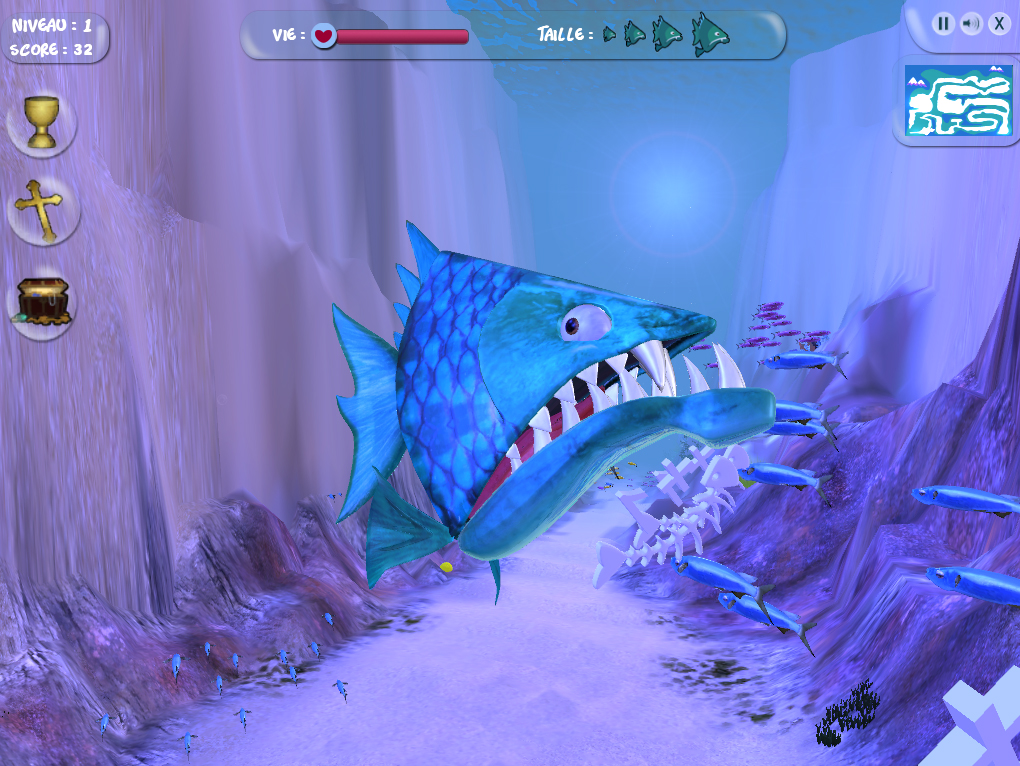
\includegraphics[width=0.8\linewidth]{images/voracy_fish}
\caption{Capture d'écran du jeu "Voracy Fish" de GENIOUS.}
\label{fig:voracy_fish}
\end{figure}

MOJOS se différencie d'un moteur jeu "normal" dans la mesure où il propose
un rééquilibrage dynamique de la difficulté afin de garder le patient dans
ce que Mihály Csíkszentmihályi nomme "Le Flux"\cite{flow}. Il y a en plus un suivi possible 
des performances du patient par son médecin.

\subsubsection{Hammer \& Planks}
Hammer \& Planks (voir figure \ref{fig:hammer_planks}), jeu en développement par NaturalPad, se veut à la fois 
ludique et thérapeutique. Il est donc possible de contrôler le jeu via différents contrôleurs, dont une manette ou une Kinect.

\begin{figure}[h!]
\centering
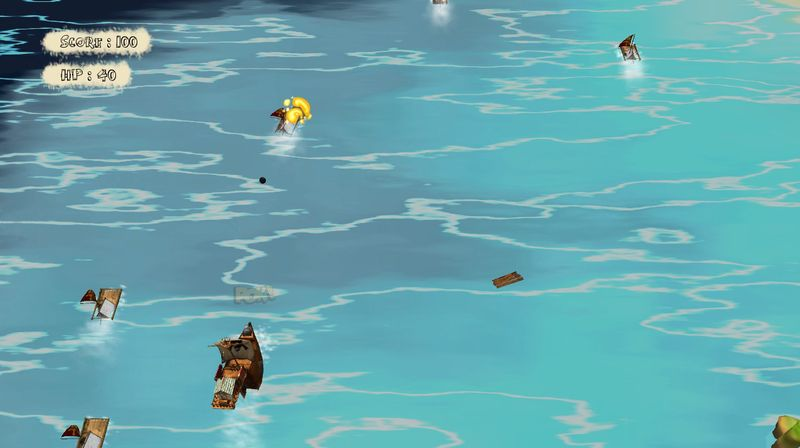
\includegraphics[width=1.0\linewidth]{images/hammer_and_planks}
\caption{Capture d'écran du jeu "Hammer and Planks" de 
NaturalPad.}
\label{fig:hammer_planks}
\end{figure}

Parmi les points intéressants il est offert ici la possibilité de modifier certains
paramètres du jeu par l'intermédiaire d'un terminal annexe, l'idée étant de
permettre à un spécialiste de rééquilibrer le jeu selon les besoins de son
patient.

	
% ------------------------------------------------------------------------------  
% ------------------------------------------------------------------------------  
% ------------------------------------------------------------------------------  
	
	\chapter{Propositions}
	
		\section{Solutions}
    \subsection{Outils et technologies} 
    \subsection{Outils et technologies} 
\subsubsection{Pourquoi la Kinect?}
La Kinect est, d'après ce que nous venons de voir, un outil peu cher, 
très disponible car grand-public, et utilisable sur toutes les plateformes
majeures, avec des bindings pour la majorité des langages de programmation 
bien-connus.

\subsubsection{Pourquoi Unity?}
Nous avons eu quelques réticences par rapport à Unity, étant donné que c'est 
un outil fermé qui n'est utilisable que sous Windows et Mac. Pourtant nous ne 
pouvons nier les résultats obtenus avec en de très courtes durées. C'est
un outil parfait pour le prototypage rapide et, vu qu'il s'agit à la base d'un
moteur de jeu, il permet facilement d'ajouter des aspects jeu à notre projet.

\subsubsection{Pourquoi Zigfu?}
Étant donnée les choix de la Kinect et de Unity il n'y avait pas beaucoup d'options
pour la bibliothèque de middleware. Des binding OpenNI pour Unity existaient
à une époque, mais ne sont plus maintenus depuis 2 ans~: en effet c'est de ce
projet qu'est parti Zigfu pour OpenNI\cite{zigfu_branch}.

    
		\subsection{Cahier de charges / user stories} 		%---GEOFFREY--
		
		MAINTENANT QU'ON A FINI NOTRE ETUDE DE TERRAIN ON PROPOSE L'APPLICATION PARFAITE 
		
		ou pas - m'enfin bref.
		
		- faire les 4 exerices dont on a parlé
		-- pourquoi ces 4 là? Pourquoi pas les autres?
		--- problème pour les jambes (distances, bizarreté)
		--- problème pour mesurer la rotation (extrapolés)
		--- problème pour mesurer les doigts 
		
		- fournir un 'score' plus précis que celui que propose la FM
		-- l'angle exacte auquel on est arrivé
		-- savoir combien on a progrésé
		
		- tester si le patient fait un mouvement 'illegal'
		-- le prevenir
		-- recommencer le teste
		
		
		- gamification
		-- environnement agréeable
		-- ??? pourquoi ça s'applique mal
		--- mieux les truc répétifs (le FM on le fait genre une fois par semaine!)
		--- cela étant, les notions de feedback, d'intéractions 
			'meaningful play = integrated + discernable' (Rules of Play) les actions ont un 
			impact et on sait lequel. 
		
		\section{Mise en oeuvre} 	%	---WILLIAM + GEOFFREY--

		Grapher
		- FailGrapher (montre la croix en plus de la progression)
		
		Multicamera
		
		ExerciseMonitor
		- FlexionMontior et compagnie
		
		Machine à états (on aime bien les trucs visuels dans les rapports)
		
		\section{Limites}%		---GEOFFREY--
			\subsection{Test de Fugl Meyer}
Comme indiqué précédement, ce test constitue le standard en la matière et on ne peut donc pas passer à coté en premier lieu.
Cependant, les exerices et le test en lui-même ont pour vocation de rapidement évaluer les capacités ou déficience
du patient. La plupart des exercices du test ne dure ainsi que quelques secondes. Cela, couplé au fait que tous les 
médecins ne font pas faire chaque partie du test, ni surtout dans le même ordre, implique une interface permettant de 
choisir quelle partie du test exécuter. Le problème que l’on peut voir, c'est qu'au final on passerait 
bien plus de temps dans cette interface que dans les "jeux" à proprement parler.

\paragraph{}
D'après notre observation de la réalisation d'un test avec une jeune patiente, celle-ci focalise 
beaucoup son regard sur les membres concernés par l'exercice. Il nous a été confirmé que c'était un fait fréquent
chez les patients, notamment en début de réhabilitation. Pour cette raison, il n'est pas possible de leur
demander de regarder un écran tant qu'ils exécutent un mouvements leur demandant un effort particulier.
On retrouve aussi un test qui demande au patient de fermer les yeux.

\paragraph{}
Par ailleurs, les tests distaux (mains et poignets) nécessitent une précision que ne permet pas la kinect.
Pour les mains, les test sont évalués de manière “tactile” (tests de résistance, de préhension) pour la plupart, 
avec peu de différence visuelle entre une évaluation 0 et 2. L’utilisation de la Kinect semble alors 
peu pertinente pour cette partie de l’évaluation..

\paragraph{}
On rappellera le problème de "l'effet plateau", du à un manque de granularité de l'évaluation, et la possibilité
d'obtention d'un score maximal sans pour autant avoir atteint une guérison complète. Rappelons aussi la variabilité
des évaluations par les praticiens, et le problème que cela implique de trouver une manière "neutre" d'interprêter
les mouvements du patient.
Enfin, les gestes demandés par FM sont très précis et non modifiables. Cela peut limiter les possibilités de “gamification”.
		
			\subsection{Zigfu}	
		Zigfu c'est de la merde!!!!
		- ils profitent d'un projet open source
		- ils apportent rien
		- pas de docs
		- code mal écrit
		- la moitié des samples marchent pas pour WILLIAM :D
		
		\subsection{Capteur Kinect}
		La Kinect en générale ??????  et un apport du Kinect pas évident.
		- les rotations (pas récupérés par la SDK de Microsoft => déduits)
		  -- est il possible de les "voir" directement?  
Notons aussi que certains exo du test du Fugl Meyer ne peuvent pas être fait/interprêtés par la kinect, il en résulte
un test du Fugl Meyer tronqué et plus long à réaliser.
		- les mouvement distaux (pas de capture des doits individuelles)

\paragraph{Remarque :\\}
Chose à prendre en compte : ne pas imaginer un feedback "trop incitateur". Cad : si un patient n'arrive pas à 
réaliser un mouvement complet, le feedback ne doit pas l'inciter à forcer + qu’il peut raisonnablement le faire.
		
		\section{Ouverture}	%	---GEOFFREY--
		
		- alternatifs: ARAT = test fonctionnel et non de déficience (le médecin il le vendait TROP)
Cela amène à une reflexion, qui serait de plutôt orienter un éventuel développement futur (hors cadre TER) vers
des exercices de rééducation ou autres types de test plutôt que vers les 'exercices' du test de Fugl Meyer.
		- projet de stage avec NaturalPad: faire de extraction de squelette moins nul
		- possibilités de concurence avec Zigfu vu qu'il a juste repris 
		- la gamification est plus pertinente / adapté aux exercices de rehabiliation 
		-(Idée : interface orale?)
		
    \section{Références}
    \chapter{Références}
\paragraph{Ressources web}
  \begin{itemize}
	\item docs.unity3d.com/
    \item zigfu.com
    \item www.openni.org/
    \item www.nightmarekitty.com 
    \item www.creativeapplications.net
  \end{itemize}
  
\paragraph{Articles}
  \begin {itemize}
    \item Evaluation of the disabilities of hemiplegic patients [M.-C. Gellez-Leman et al.] \label{ref_analyse_litterature}
    \item LEAPS Fugl-Meyer Instructions
  \end{itemize}
        
        
        
%http://www.creativeapplications.net/tutorials/guide-to-camera-types-for-interactive-installations/
    
\part{Annexes}
	\chapter{Fiche d'évaluation du score de FM pour les membres supérieurs} \label{evaluation_FM}
	%TODO \includegraphics[scale=1]{scan_fichie_evalation.jpngif}
\end{document}
